\documentclass[12pt]{article}

\usepackage{enumerate}
\usepackage{rotating}
\usepackage{multicol}
\usepackage{multirow}
\usepackage{graphicx}
\usepackage{fullpage}
\usepackage{subfigure}
\usepackage{setspace}
\usepackage{listings}
\usepackage{lastpage}
\usepackage{amsmath}
\graphicspath{{./images/}}

% for references
\usepackage[pagebackref=false,colorlinks,linkcolor=blue,citecolor=magenta]{hyperref}
\usepackage[nottoc]{tocbibind}
\usepackage{fancyhdr}
\setlength{\headsep}{25pt}

\pagestyle{fancy}
\fancyhf{}
\lhead{\lr{Digital Image Processing}}
\rhead{تمرین پنجم}
\cfoot{صفحه \thepage\ از \pageref{LastPage}}
\lfoot{نیمسال مهر 00-99}
\rfoot{حمیدرضا ابوئی مهریزی}


% xepersian
\usepackage[extrafootnotefeatures]{xepersian}
\settextfont[Scale=1.4]{B Nazanin}
\setlatintextfont{Times New Roman}

\renewcommand{\labelitemi}{$\bullet$}

\begin{document}
	\doublespacing
	\begin{titlepage}
		\paragraph*{}
		\centering
			
			
			{\small به نام او}\\
			\vspace{1cm}
			\includegraphics[width=0.12\paperwidth]{aut.png}
			\hspace{1cm}
			\includegraphics[width=0.15\paperwidth]{DIP}
			\hspace{1cm}
			\includegraphics[width=0.12\paperwidth]{bme}\\
			\vspace{2cm}
			{\Huge پردازش تصویر}\\
			\vspace{2cm}
			{\large استاد : دکتر حامد آذرنوش}\\
			\vspace{0.5cm}
			{\small  دانشجو :‌ حمیدرضا ابوئی}\\
			\vspace{0.5cm}
			{\small شماره دانشجویی : 9733002}\\
			\vspace{0.5cm}
			{\small تمرین پنجم}\\
			\vfill
			{\tiny نیمسال مهر 00-99}
	\end{titlepage}
	\thispagestyle{plain}
	\tableofcontents
	\newpage
	%\onehalfspacing
	\doublespacing
	\section{سوال اول}
		\subsection{توضیحات تکمیلی روند کد}
	روش های زیادی برای دریافت نقاط وجود دارد یکی از روش ها که در کد موجود است، دریافت مختصات نقاط کلیک شده روی تصویر در محیط 
	\lr{matplotlib}
	و سپس تغییر تصویر پس زمینه است.
	بدین صورت که پس از انتخاب ۳ نقطه تصویر جدید ظاهر میشود و پس از انتخاب سه نقطه ی دیگر، به سراغ حل مساله میرود.
	
	حل این مساله با توجه به ۶ نقطه ی انتخابی و 6 معادله 6 مجهول و یا به صورت آسان تر با استفاده از تابع پیش فرض 
	\lr{getAffineTransform}
	قابل انجام است و درایه های تابع تبدیل مورد نظر ما را به ما میدهند . که با اعمال آن روی تصویر اول میتوان آن را به تصویر دوم تبدیل کرد.
		\subsection{ورودی برنامه}
		\includegraphics[width=5cm]{inputs/mrif}
		\includegraphics[width=8cm]{inputs/mris}\\
		و سه نقطه از تصویر اول و ۳ نقطه از تصویر دوم 
		\subsection{خروجی برنامه}
		
		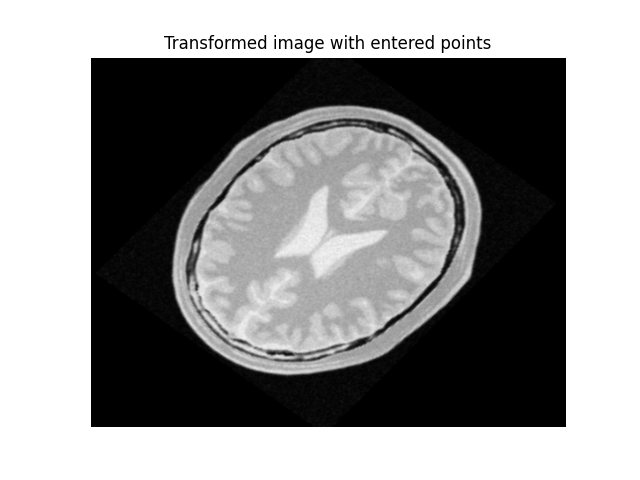
\includegraphics[width=10cm]{1}\\

		\newpage
		
			\doublespacing
		\section{سوال دوم}
		\subsection{توضیحات تکمیلی روند کد}
		این کد با وجود تلاش های بسیار به دلیل کمبود وقت متاسفانه پیاده سازی نشد اما توضیحاتی که از تلاش ها و مطالعات به دست آمد در ادامه بیان می‌شود .
		۱ روش این سوال بدین صورت است که ابتدا ابعاد تصویر را به ابعاد مربع توان 2 در می آوریم مانند 512*512  و یا 1024*1024 (تصویر ما ۲ پیکسل از طرفین کادر سفید دارد که با حذف آن ، به ابعاد ۵۱۲*۵۱۲ میرسیم) حال شروع به نصف کردن تصویر به 4 قسمت میکنیم . حال شرطی را که برای یافتن سگمنت های متفاوت روی تصویر داریم را چک میکنیم . این شرط میتواند به صورت زیر باشد 
		
		۱- شرط تفاوت حداقل و حداکتر مقدار شدت کمتر از یک عدد مانند ۴۰ 
	
		۲- شرط حداکثر میزان انحراف از معیار مثلا ۲۰ 
		
		حال با بررسی شروط ، اگر آن قسمت شرط ها را با موفقیت به انجام میرساند ، نیازی به تقسیم مجدد وجود ندارد ولی اگر آن قسمت شرط ها را رعایت نکرد مجددا به ۴ قسمت تقسیم میکنیم و این لوپ را انقدر ادامه میدهیم تا ۱ - شرط ها برای تمام قسمت ها رعایت شوند یا ۲ - به حداقل سایز مورد نظر برسیم (در این سوال ۲*۲ - 4*4 - 8*8 و یا 16*16) 
		حال ما این قسمت ها را داریم و میخواهیم سراغ ترکیب قسمت های مشابه برویم . 
		
		حال برای یافتن شباهت ها باید همسایگی ها را بیابیم و آن ها را با شروط یاد شده بسنجیم تا ببینیم که آیا به هم مربوط هستند یا خیر و اگر مربوط بودند هر دو را ترکیب میکنیم .
		
		البته مشکلات و راه حل هایی برای این مراحل وجود دارد که تعدادی از آن ها در ادامه ذکر خواهد شد.
		اولین مشکل یافتن همسایگی هاست. ابن مشکل یکی از بزرگ ترین مشکلات محسوب می‌شود. 
		
		با دو نگاه این موضوع را بررسی خواهیم کرد:
		
		۱- این که ما برای یافتن قسمت های مختلف تصویر از متد نام گذاری طولی استفاده کنیم یعنی اگر تصویر ما ۵۱۲ در ۵۱۲ باشد و حداقل ابعاد ما برای یک قطعه ۴ باشد برای یافتن آن باید از طریق آدرس دهی به صورت 
	\lr{	subimage[0,1,2,1,2,1,1]    }
		استفاده شود. همسایه یابی در این جور آدرس دهی قابل انجام است اما شرط های دقیقی دارد برای مثال اگر همسایگی ۴ تایی اطراف هر قسمت را در نظر بگیریم، هر قسمت باید با پیکسل سمت راست و پایین خود مقایسه و احیانا ترکیب شود . بدین منظور این قسمت ما باید با دو قسمت زیر بررسی شود:
		
	\lr{subimage[0,1,2,1,3,0,0] , subimage[0,1,2,1,2,1,3]}
	در صورت استفاده از این روش، باید کلا تصویر را به قطعات ۱۶ در ۱۶ تقسیم کنیم تا این نوع نام گذاری ما و شرط های مد نظر قابل پیاده سازی باشد.
		۲- برای هر قسمت ، یک عدد در نظر بگیریم و یک تصویر بسازیم که هر پیکسل آن نشان دهنده ی قسمت مربوط به آن پیکسل در تصویر متناظر آن خواهد بود یعنی یک تصویر مشابه تصویر اصلی داریم که به جای نگهداری شدت هر پیکسل، قسمت مربوط به آن را در خود نگه می دارد. حال با تقسیم کردن متوالی تصویر و چک کردن شرط مرحله ی جداسازی را به پایان می‌بریم . حال برای یافتن قسمت های همسایه، در هر قسمت تمام پیکسل ها را چک میکنیم و قسمت های موجود در همسایگی ۴ (و یا همسایگی ۸) آن را می یابیم . سپس آن ها را مقایسه کرده و اگر هر دو با هم در شرط ما صدق میکردند، مقدار آن ها را یکی میکنیم یعنی با هم ترکیب کردیم و در خروجی میتوانیم این ماتریس دوم را نمایش دهیم.
		
		
		
		
		
		\subsection{ورودی برنامه}
		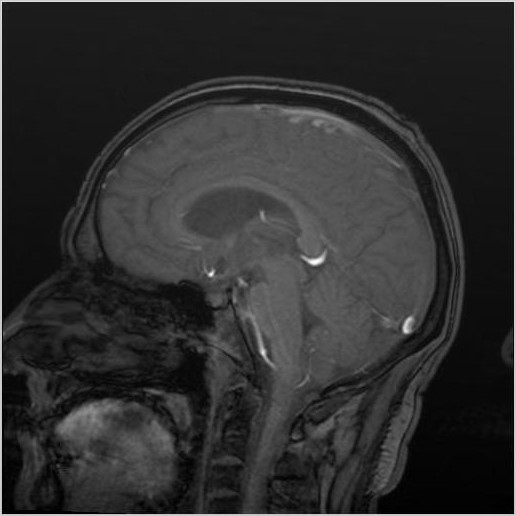
\includegraphics[width=5cm]{inputs/fMRI}
		\subsection{خروجی برنامه}
		
		
		
		\newpage
		\section{سوال سوم}
		\subsection{توضیحات تکمیلی روند کد}
		با یک توضیح مختصر راجع به تبدیل 
		\lr{Hough}
		به سراغ حل مساله می‌رویم.
		
		در این تبدیل خطوط که در صفحه وجود دارند به جای این که در مختصات کارتزین مرود بررسی قرار گیرند (به دلیل این که گستره ی آن نامحدود است) در مختصات قطبی مورد بررسی قرار میگیرند. نقاط تلاقی این خطوط همان خطوطی هستند که در تصویر وجود دارند. هر چه نقطه تلاقی این دو بیشتر باشند نشان دهنده ی این است که در تصویر ما چه تعداد نقطه از این خط عبور کرده اند .
		
		حال ، اگر ما این الگوریتم را در نصویر پیاده سازی کنیم، خطوطی که به دست می آید بسیار زیاد است و این نشان دهنده ی آن است که نویز نسبتا زیادی روی تصویر داریم بنابراین ما تصویر را باید با یک فیلتر گوسین (یا میانه ) فیلتر کنیم تا اثر نویز های مخرب کمینه شود.
		نکته ی قابل ذکر دیگر استفاده از 
		\lr{HoughlinesP}
		است که به ما به جای مختصات خط، مختصات پاره خط یافت شده را باز میگرداند .
		البته هر کدام از این توابع ورودی های زیادی دارند که سعی شد با سعی و خطا مقادیری مناسب برای آن یافت شود.
		
		در مورد سلول ها نیز با روش مشابه ابتدا دایره ها ی یافته شده از تصویر به همراه شعاع آن ها یافته شد و با استفاده از یک شرط ساده که مربوط به شعاع دایره ها بود گلبول های سفید که بزرگ تر از سلول های قرمز خونی هستند قابل تشخیص هستند . البته مبرهن است که در این قسمت نیز ابتدا باید نویز تصویر گرفته شود تا خروجی مناسبی داده شود.
		
		
		
		\subsection{ورودی برنامه}
		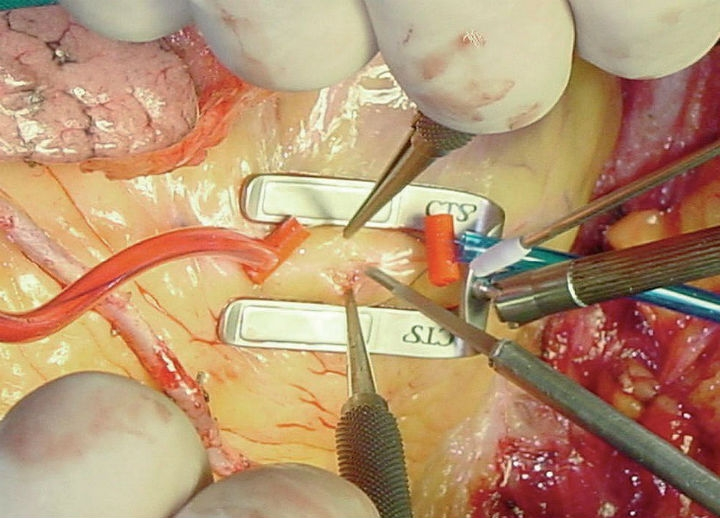
\includegraphics[width=5cm]{inputs/surgery}
		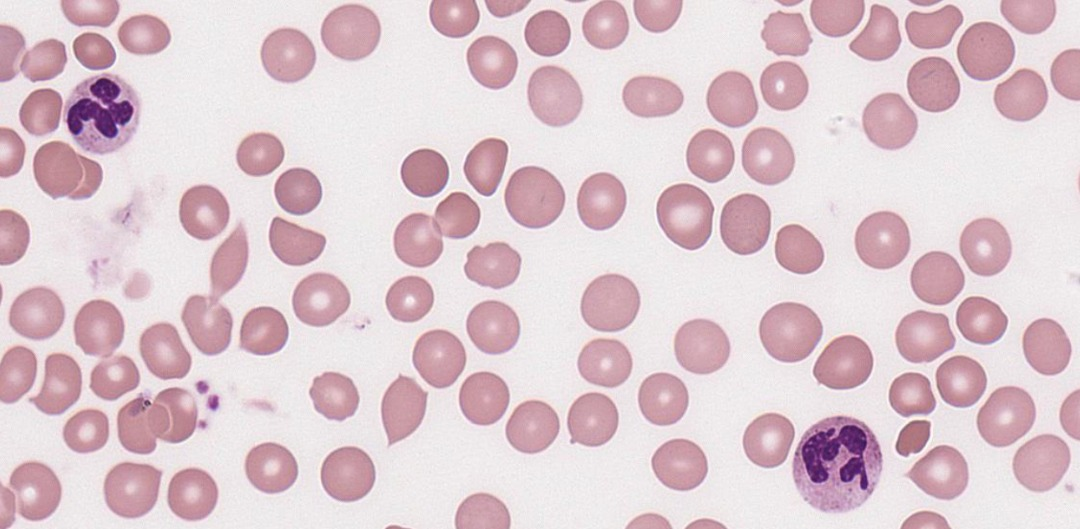
\includegraphics[width=8cm]{inputs/redcell}
		\subsection{خروجی برنامه}
		
		\includegraphics[width=15cm]{3}\\
		\includegraphics[width=15cm]{3-1}
		
		\newpage
		
		\section{سوال چهارم}
		\subsection{توضیحات تکمیلی روند کد}
		\begin{itemize}
			\item 
			\lr{sobel} :
			 این فیلتر که به صورت 
			\begin{bmatrix}
				+1&+2&+1\\
				0&0&0\\
				-1&-2&-1\\
			\end{bmatrix}
		و یا 
		\begin{bmatrix}
			-1&0&+1\\
			-2&0&+2\\
			-1&0&+1\\
		\end{bmatrix}
	روی تصویر اعمال می شود که لبه های عمودی و افقی را می یابد البته در کد نوشته شده به صورت جمع دو نتیجه برای نمایش لبه های افقی و عمودی استفاده شده است. 
	\item 
	\lr{prewit} :
	مانند فیلتر سوبل است اما با این تفاوت که فیلتر زیر به کار رفته است 
	\begin{bmatrix}
		+1&+1&+1\\
		0&0&0\\
		-1&-1&-1\\
	\end{bmatrix}
	و 
	\begin{bmatrix}
		-1&0&+1\\
		-1&0&+1\\
		-1&0&+1\\
	\end{bmatrix}

	\item
	\lr{LoG (Laplacian of Gaussian filter )} :
	کارکرد این فیلتر از روی اسمش پیداست و عموما تابع آن به صورت زیر است:
		\begin{bmatrix}
		0&0&1&0&0\\
		0&1&2&1&0\\
		1&2&-16&1&0\\
		0&1&2&1&0\\
		0&0&1&0&0\\
		
	\end{bmatrix}
	
	\item 
	\lr{canny} :
	این الگوریتم عموما با ۴ مرحله انجام می‌شود. ۱ - کاهش نویز ۲ - یافتن گرادیان شدت در تصویر ۳ - حذف اضافات غیر لبه ها ۴ - یافتن لبه های واقعی با استفاده از آستانه گذاری .
	\item 
	\lr{roberts} :
	این فیلتر قدیمی نیز حاصل اعمال دو فیلتر زیر  روی تصویر می‌باشد .
	\begin{bmatrix}
		1&0\\
		0&-1\\
	\end{bmatrix}
و
	\begin{bmatrix}
		0&1\\
		-1&0\\
	\end{bmatrix}
		


		\end{itemize}
		
		\subsection{ورودی برنامه}
		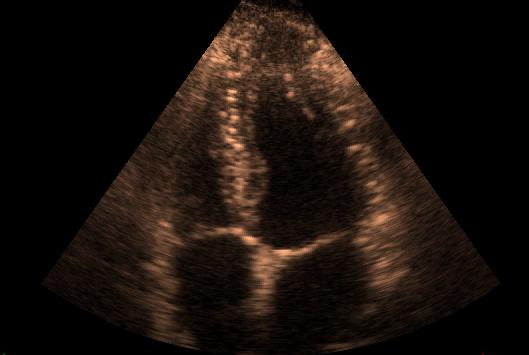
\includegraphics[width=5cm]{inputs/sonography}
		\subsection{خروجی برنامه}
		\includegraphics[width=15cm]{4}

\end{document}
